\begin{frame}
\frametitle{Creare Un Device Logico}
\begin{columns}

\column{.6\textwidth}

\begin{itemize}
\item Per interagire con il device fisico selezionato, dobbiamo creare una device logico
\item Quando creiamo il device logico, indichiamo la creazione di una coda per eseguire comandi grafici
\item Quando creiamo il device logico, indichiamo la creazione di una coda per eseguire comandi di presentazione
\item Una volta creato il device logico, possiamo ottenere le code richieste
\item Se una coda supporta sia operazioni grafiche che di presentazione, possiamo usare quella coda singolarmente
\end{itemize}

\column{.2\textwidth}

\begin{figure}[ht]
    \centering
    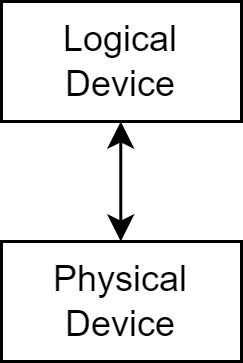
\includegraphics[scale=0.2]{images/SlidesInitializingVulkan/LogicalDevice.png}
\end{figure}

\end{columns}
\end{frame}
